\documentclass[]{article}
\usepackage{enumitem,amssymb,tikz,siunitx}
\usetikzlibrary{calc,matrix, arrows.meta, positioning, decorations,decorations.markings, math}
\newlist{todolist}{itemize}{2}
\setlist[todolist]{label=$\square$}
\usepackage{pifont}
\newcommand{\cmark}{\ding{51}}%
\newcommand{\xmark}{\ding{55}}%
\newcommand{\done}{\rlap{$\square$}{\raisebox{2pt}{\large\hspace{1pt}\cmark}}%
	\hspace{-2.5pt}}
\newcommand{\wontfix}{\rlap{$\square$}{\large\hspace{1pt}\xmark}}

%opening
\title{Proyecto Assembler ARM Cortex M0+}
\author{Santiago Calligari, Gerónimo Nestares}
\begin{document}
\maketitle
\section*{Preambulo}
\textbf{\scriptsize{Bitacora. (1/6/2022)}}\\
Se nos presento la idea y oportunidad de crear un programa en el lenguaje ensamblador de la placa de desarrollo Raspberry Pi Pico. \\
Este proyecto cuenta como el proyecto final del cuatrimestre y este archivo, como el historial, conjunto con git de nuestra historia escribiendo el codigo y entendiendo ensamblador de ARM.	
\section*{Hoja de ruta}
Para generar senos contando pura y exclusivamente con ondas digitales podemos contar con dos formas, voy a proceder a comentar la primera, PWM o modulación por ancho de pulsos.\\
\section*{Modulación Por Ancho de Pulsos}
\textbf{\scriptsize{Voltajes Arbitrarios A Partir de Valores Fijos}}

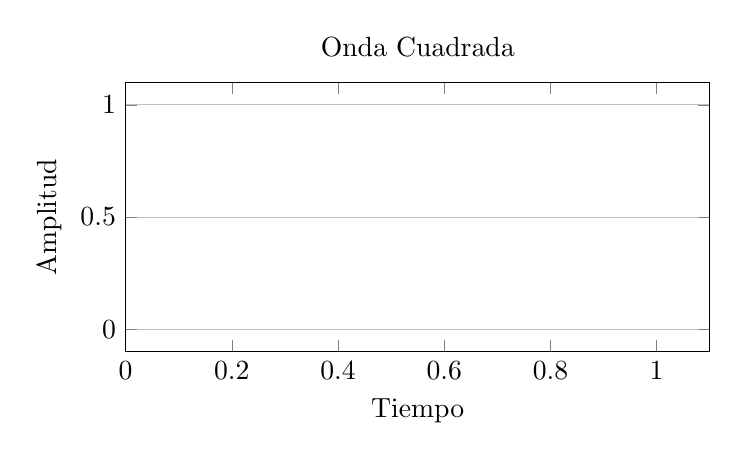
\begin{tikzpicture}
	\begin{axis}[ymajorgrids=true,xmin=0,width=9cm,height=5cm,
		title=Onda Cuadrada ,xlabel={Tiempo},ylabel=Amplitud, 
		ytick={0,1}]
		\foreach \x in {0.4,0.8,...,4} { \draw[blue] (\x,0)--(\x,2)--(\x+0.2,2)--(\x+0.2,0); }
		\foreach \x in {4.4,4.8,5.2} { \draw[red] (\x,0)--(\x,-2)--(\x+0.2,-2)--(\x+0.2,0); }
	\end{axis}
\end{tikzpicture}



\end{document}
